\lesson{12}{May 14 2022 Sat (21:49:09)}{The Laws of Sin and Cos}
\label{les_12:the_laws_of_sin_and_cos}

The triangle in Figure \ref{fig:non_right_triangle} is a non-right triangle
since none of its angles measure $90^{\circ}$. We'll start by deriving the
\textbf{Laws of Sin and Cos} so that we can study non-right triangles.

\begin{figure}[htpb]
	\centering

	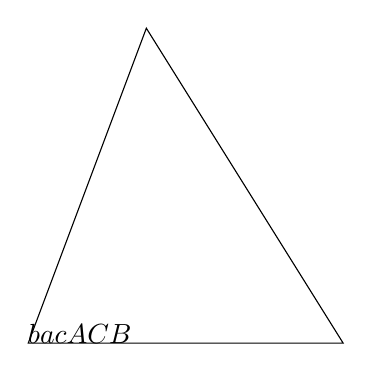
\begin{tikzpicture}
		\coordinate (a) at (0,0);
		\coordinate (b) at (4,0);
		\coordinate (c) at (1.5,4);

		\draw (a) -- (c) -- (b) -- cycle;

		\tkzLabelSegment (a,c) {$b$};
		\tkzLabelSegment (c,b) {$a$};
		\tkzLabelSegment[below=2pt](a,b){$c$};

		\tkzMarkAngle[mark=none](b,a,c);
		\tkzLabelAngle[pos=0.5](b,a,c){$A$};

		\tkzMarkAngle[mark=none](a,c,b);
		\tkzLabelAngle[pos=0.5](a,c,b){$C$};

		\tkzMarkAngle[mark=none](c,b,a);
		\tkzLabelAngle[pos=0.5](c,b,a){$B$};
	\end{tikzpicture}

	\caption{}
	\label{fig:non_right_triangle}
\end{figure}

\subsection*{The Law of Sin}
\label{sub_sec:the_law_of_sin}

To derive the \textbf{Law of Sin}, let's construct a segment $h$ in the
triangle, which connects the vertex of angle $C$ to the side $c$. This segment
should be perpendicular to side $c$ and is called a \textit{height} of the
triangle. See Figure \ref{fig:non_right_triangle_2}.

\begin{figure}[htpb]
	\centering

	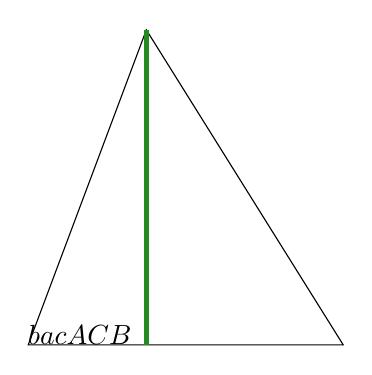
\begin{tikzpicture}
		\coordinate (a) at (0,0);
		\coordinate (b) at (4,0);
		\coordinate (c) at (1.5,4);
		\coordinate (d) at (1.5,0);

		\draw (a) -- (c) -- (b) -- (d) -- (b) -- cycle;

		\draw[ultra thick,ForestGreen] (c) -- (d);

		\tkzLabelSegment (a,c) {$b$};
		\tkzLabelSegment (c,b) {$a$};
		\tkzLabelSegment[below=2pt](a,b){$c$};
		\tkzMarkAngle[mark=none](b,a,c);
		\tkzLabelAngle[pos=0.5](b,a,c){$A$};
		\tkzMarkAngle[mark=none](a,c,b);
		\tkzLabelAngle[pos=0.5](a,c,b){$C$};
		\tkzMarkAngle[mark=none](c,b,a);
		\tkzLabelAngle[pos=0.5](c,b,a){$B$};
	\end{tikzpicture}

	\caption{}
	\label{fig:non_right_triangle_2}
\end{figure}

The segment $h$ splits the triangle into two right triangles on which we can
apply what we know about right triangle trigonometry. See Figure
\ref{fig:non_right_triangle_split_into_two_right_triangles_1}

\begin{figure}[htpb]
	\centering

	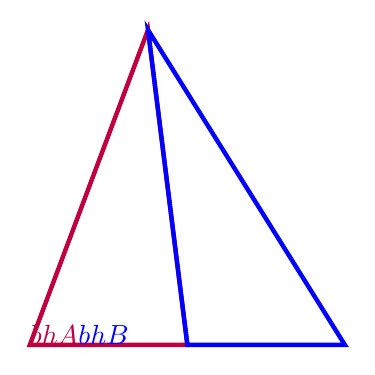
\begin{tikzpicture}
		\coordinate (a1) at (0,0);
		\coordinate (b1) at (2,0);
		\coordinate (c1) at (1.5,4);

		\coordinate (a2) at (2,0);
		\coordinate (b2) at (4,0);
		\coordinate (c2) at (1.5,4);

		\draw[ultra thick,purple] (a1) -- (c1) -- (b1) -- cycle;
		\draw[ultra thick,blue] (a2) -- (c2) -- (b2) -- cycle;

		\tkzLabelSegment (a1,c1) {{\color{purple}$b$}};
		\tkzLabelSegment (b1,c1) {{\color{purple}$h$}};

		\tkzMarkAngle[mark=none,size=2.5mm](b1,a1,c1);
		\tkzLabelAngle[pos=0.5](b1,a1,c1){{\color{purple}$A$}};

		\tkzLabelSegment (c2,b2) {{\color{blue}$b$}};
		\tkzLabelSegment[right=0.15](c2,a2){{\color{blue}$h$}};

		\tkzMarkAngle[mark=none,size=2.5mm](c2,b2,a2);
		\tkzLabelAngle[pos=0.5](c2,b2,a2){{\color{blue}$B$}};
	\end{tikzpicture}

	\caption{}
	\label{fig:non_right_triangle_split_into_two_right_triangles_1}
\end{figure}

We can use the $2$ right triangles to obtain expressions for both $\sin (A)$ and
$\sin (B)$.
\[ \sin (A) = \frac{h}{b} \textrm{ and } \sin (B) = \frac{h}{a} \].
We can now solve both of these equations for $h$:
\begin{align*}
	\qquad         & \sin (A) = \frac{h}{b} \textrm{ and } \sin (B) = \frac{h}{a} \\
	\implies\qquad & h = b\sin(A) \textrm{ and } h = a\sin (B)
	.\end{align*}

Now, since both of the $h$'s represent the length of the same segment, they are
equal. By setting $h$'s equal to each other we obtain the following:
\[ b\sin (a) = a\sin (B) \].
This equation provides us with what is known as the \textbf{Law of Sin}.
Typically, the law is written in terms of ratios. If we divide both sides by
$a \times b$, we obtain the following:
\begin{align*}
	\qquad         & b\sin (A) = a\sin (B)                                       \\
	\implies\qquad & \frac{b\sin (A)}{a \times b} = \frac{a\sin (B)}{a \times b} \\
	\implies\qquad & \frac{\sin (A)}{a} = \frac{\sin (B)}{b}
	.\end{align*}

\begin{definition}[Law of Sines]
	\label{def:law_of_sines}

	If a triangle's sides and angles are labeled like the triangle in Figure
	\ref{fig:law_of_sines}, then:

	\begin{figure}[H]
		\centering

		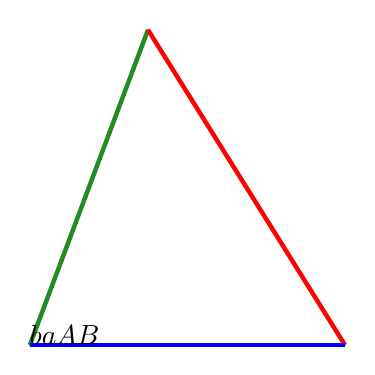
\begin{tikzpicture}
			\coordinate (a) at (0,0);
			\coordinate (b) at (4,0);
			\coordinate (c) at (1.5,4);

			\draw (a) -- (c) -- (b) -- cycle;

			\draw[ultra thick,ForestGreen] (a) -- (c);
			\draw[ultra thick,red] (c) -- (b);
			\draw[ultra thick,blue] (a) -- (b);

			\tkzLabelSegment (a,c) {$b$};
			\tkzLabelSegment (c,b) {$a$};

			\tkzMarkAngle[mark=none](b,a,c);
			\tkzLabelAngle[pos=0.5](b,a,c){$A$};
			\tkzMarkAngle[mark=none](c,b,a);
			\tkzLabelAngle[pos=0.5](c,b,a){$B$};
		\end{tikzpicture}

		\caption{}
		\label{fig:law_of_sines}
	\end{figure}

	\[ \frac{\sin (A)}{a} = \frac{\sin (B)}{b} \].
	This is an \textbf{identity} since it is true for \textit{all} triangles.
\end{definition}

\begin{exc}[Solution \ref{sol:law_of_sines}]
  \label{exc:law_of_sines}

  Find all the missing angles and side-lengths of the triangle given in Figure
  \ref{fig:law_of_sines_with_missing_angles_and_side_lengths_1} (The triangle is
  not necessarily drawn to scale.)

	\begin{figure}[H]
		\centering

		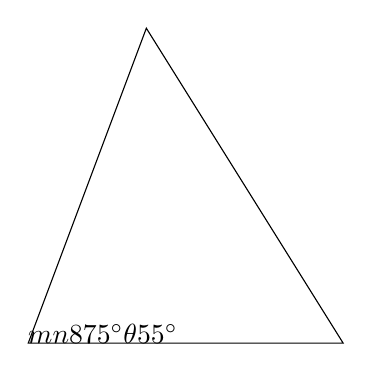
\begin{tikzpicture}
			\coordinate (a) at (0,0);
			\coordinate (b) at (4,0);
			\coordinate (c) at (1.5,4);

			\draw (a) -- (c) -- (b) -- cycle;

			\tkzLabelSegment (a,c) {$m$};
			\tkzLabelSegment (c,b) {$n$};
      \tkzLabelSegment[below=2pt](a,b){$8$};

			\tkzMarkAngle[mark=none](b,a,c);
			\tkzLabelAngle[pos=0.5](b,a,c){$75^{\circ}$};
			\tkzMarkAngle[mark=none](c,b,a);
			\tkzLabelAngle[pos=0.5](c,b,a){$\theta$};
			\tkzMarkAngle[mark=none](a,c,b);
			\tkzLabelAngle[pos=0.5](a,c,b){$55^{\circ}$};
		\end{tikzpicture}

		\caption{}
		\label{fig:law_of_sines_with_missing_angles_and_side_lengths_1}
	\end{figure}
\end{exc}

% subsection the_law_of_sin (end)

\newpage

\subsection*{The Law of Cos}
\label{sub_sec:the_law_of_cos}

To derive the \textbf{Law of Cos}, let's start with a generic triangle and draw
the height, $h$, just as we did when we derived the Law of Sin. See Figure
\ref{fig:non_right_triangle_3}.

\begin{figure}[htpb]
	\centering

	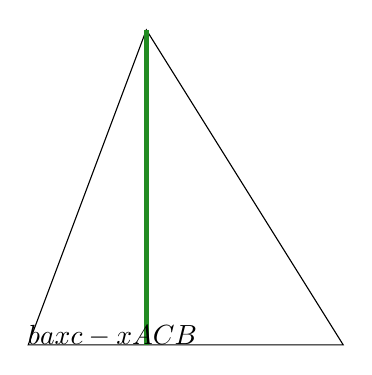
\begin{tikzpicture}
		\coordinate (a) at (0,0);
		\coordinate (b) at (4,0);
		\coordinate (c) at (1.5,4);
		\coordinate (d) at (1.5,0);

		\draw (a) -- (c) -- (b) -- (d) -- (b) -- cycle;

		\draw[ultra thick,ForestGreen] (c) -- (d);

		\tkzLabelSegment (a,c) {$b$};
		\tkzLabelSegment (c,b) {$a$};
		\tkzLabelSegment[below=2pt](a,d){$x$};
		\tkzLabelSegment[below=2pt](b,d){$c-x$};
		\tkzMarkAngle[mark=none](b,a,c);
		\tkzLabelAngle[pos=0.5](b,a,c){$A$};
		\tkzMarkAngle[mark=none](a,c,b);
		\tkzLabelAngle[pos=0.5](a,c,b){$C$};
		\tkzMarkAngle[mark=none](c,b,a);
		\tkzLabelAngle[pos=0.5](c,b,a){$B$};
	\end{tikzpicture}

	\caption{}
	\label{fig:non_right_triangle_3}
\end{figure}

Again we want to consider the two right triangles induced by constructing the
line $h$ on the triangle given in Figure \ref{fig:non_right_triangle_3}. This
time, we want to use the two pieces that the side $c$ is split into. Let's call
the segment on the left $x$ and then the segments on the right must be $c - x$
units long. We've emphasized the two right triangles and labeled the two pieces
of side $c$ in Figure
\ref{fig:non_right_triangle_split_into_two_right_triangles_2}

\begin{figure}[htpb]
	\centering

	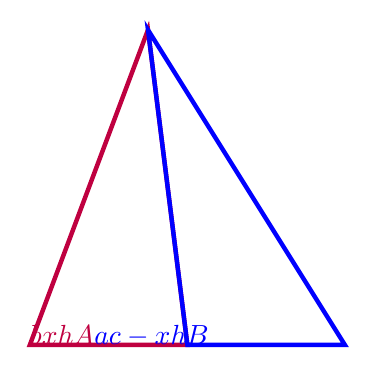
\begin{tikzpicture}
		\coordinate (a1) at (0,0);
		\coordinate (b1) at (2,0);
		\coordinate (c1) at (1.5,4);

		\coordinate (a2) at (2,0);
		\coordinate (b2) at (4,0);
		\coordinate (c2) at (1.5,4);

		\draw[ultra thick,purple] (a1) -- (c1) -- (b1) -- cycle;
		\draw[ultra thick,blue] (a2) -- (c2) -- (b2) -- cycle;

		\tkzLabelSegment (a1,c1) {{\color{purple}$b$}};
		\tkzLabelSegment[below=2pt](a1,b1){{\color{purple}$x$}};
		\tkzLabelSegment (b1,c1) {{\color{purple}$h$}};

		\tkzMarkAngle[mark=none,size=2.5mm](b1,a1,c1);
		\tkzLabelAngle[pos=0.5](b1,a1,c1){{\color{purple}$A$}};

		\tkzLabelSegment (c2,b2) {{\color{blue}$a$}};
		\tkzLabelSegment[below=2pt](a2,b2){{\color{blue}$c - x$}};
		\tkzLabelSegment[right=0.15](c2,a2){{\color{blue}$h$}};

		\tkzMarkAngle[mark=none,size=2.5mm](c2,b2,a2);
		\tkzLabelAngle[pos=0.5](c2,b2,a){{\color{blue}$B$}};
	\end{tikzpicture}

	\caption{}
	\label{fig:non_right_triangle_split_into_two_right_triangles_2}
\end{figure}

First, notice that the following is true:
\begin{align*}
  \qquad&\cos (A) = \frac{x}{b} \\
  \implies\qquad&x = b\cos (A)
.\end{align*}

Now, let's apply the Pythagorean Theorem to each of the two triangles in Figure
\ref{fig:non_right_triangle_split_into_two_right_triangles_2}. The blue triangle
on the left gives us:

\[ x^{2} + h^{2} = b^{2} \].

and we can solve this for $h^{2}$ and obtain:

\[ h^{2} = b^{2} - x^{2} \].

The blue triangle on the right gives us:

\[ (c - x)^{2} + h^{2} = a^{2} \].

and we can use the fact that $h^{2} = b^{2} - x^{2}$ to eliminate $h$ from this
equation:

\begin{align*}
  \qquad&(c - x)^{2} + h^{2} = a^{2} \\
  \implies\qquad&(c - x)^{2} + (b^{2} - x^{2}) = a^{2}
.\end{align*}

Finally, we can simplify the left side of this equation and use the fact that
$x = b\cos (A)$ to eliminate $x$:

\begin{align*}
  \qquad&(c - x)^{2} + (b^{2} - x^{2}) = a^{2} \\
  \implies\qquad&c^{2} - 2cx + x^{2} + b^{2} - x^{2} = a^{2} \\
  \implies\qquad&c^{2} - 2cx + b^{2} = a^{2} \\
  \implies\qquad&c^{2} - 3c \times b\cos (A) + b^{2} = a^{2} \\
.\end{align*}

This last equation is known as the \textbf{Law of Cosines}.

\begin{definition}[Law of Cosines]
  \label{def:law_of_cosines}

  If a triangle's sides and angles are labeled like the triangle in Figure
  \ref{fig:law_of_cosines}, then:

	\begin{figure}[H]
		\centering

		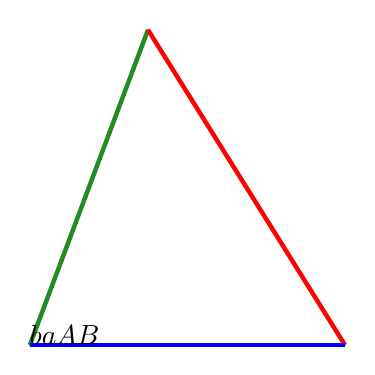
\begin{tikzpicture}
			\coordinate (a) at (0,0);
			\coordinate (b) at (4,0);
			\coordinate (c) at (1.5,4);

			\draw (a) -- (c) -- (b) -- cycle;

			\draw[ultra thick,ForestGreen] (a) -- (c);
			\draw[ultra thick,red] (c) -- (b);
			\draw[ultra thick,blue] (a) -- (b);

			\tkzLabelSegment (a,c) {$b$};
			\tkzLabelSegment (c,b) {$a$};

			\tkzMarkAngle[mark=none](b,a,c);
			\tkzLabelAngle[pos=0.5](b,a,c){$A$};
			\tkzMarkAngle[mark=none](c,b,a);
			\tkzLabelAngle[pos=0.5](c,b,a){$B$};
		\end{tikzpicture}

		\caption{}
		\label{fig:law_of_cosines}
	\end{figure}

  \[ a^{2} = b^{2} + c^{2} - 2bc \times \cos (A) \].
  This is an \textbf{identity}, since it is true for \textit{all} triangles.
\end{definition}

\begin{exc}[Solution \ref{sol:law_of_cosines}]
  \label{exc:law_of_cosines}

  Find all of the missing angles and side-lengths of the triangle given in
  Figure \ref{fig:law_of_cosines} (The triangle is not necessarily drawn to
  scale.)

	\begin{figure}[H]
		\centering

		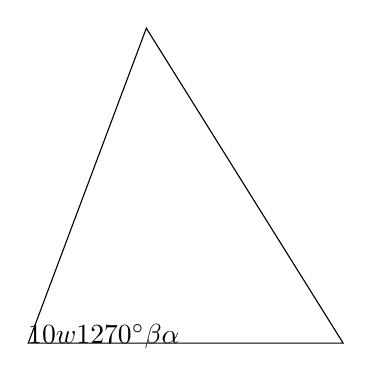
\begin{tikzpicture}
			\coordinate (a) at (0,0);
			\coordinate (b) at (4,0);
			\coordinate (c) at (1.5,4);

			\draw (a) -- (c) -- (b) -- cycle;

			\tkzLabelSegment (a,c) {$10$};
			\tkzLabelSegment (c,b) {$w$};
      \tkzLabelSegment[below=2pt](a,b){$12$};

			\tkzMarkAngle[mark=none](b,a,c);
			\tkzLabelAngle[pos=0.5](b,a,c){$70^{\circ}$};
			\tkzMarkAngle[mark=none](c,b,a);
			\tkzLabelAngle[pos=0.5](c,b,a){$\beta$};
			\tkzMarkAngle[mark=none](a,c,b);
			\tkzLabelAngle[pos=0.5](a,c,b){$\alpha$};
		\end{tikzpicture}

		\caption{}
		\label{fig:law_of_cosines}
	\end{figure}
\end{exc}

% subsection the_law_of_cos (end)

\newpage
